%%%%%%%%%%%%%%%%%%%%%%%%%%%%%%%%%%%%%%%%%%%%%%%%%%%%%%%%%%%%%%%%%%%%%%
% Colorado State University LaTeX Thesis Template and Documentation
%
% by
%   Elliott Forney
%   2017
%
% This is free and unencumbered software released into the public domain.
%
% Anyone is free to copy, modify, publish, use, compile, sell, or
% distribute this software, either in source code form or as a compiled
% binary, for any purpose, commercial or non-commercial, and by any
% means.
%
% In jurisdictions that recognize copyright laws, the author or authors
% of this software dedicate any and all copyright interest in the
% software to the public domain. We make this dedication for the benefit
% of the public at large and to the detriment of our heirs and
% successors. We intend this dedication to be an overt act of
% relinquishment in perpetuity of all present and future rights to this
% software under copyright law.
%
% THE SOFTWARE IS PROVIDED "AS IS", WITHOUT WARRANTY OF ANY KIND,
% EXPRESS OR IMPLIED, INCLUDING BUT NOT LIMITED TO THE WARRANTIES OF
% MERCHANTABILITY, FITNESS FOR A PARTICULAR PURPOSE AND NONINFRINGEMENT.
% IN NO EVENT SHALL THE AUTHORS BE LIABLE FOR ANY CLAIM, DAMAGES OR
% OTHER LIABILITY, WHETHER IN AN ACTION OF CONTRACT, TORT OR OTHERWISE,
% ARISING FROM, OUT OF OR IN CONNECTION WITH THE SOFTWARE OR THE USE OR
% OTHER DEALINGS IN THE SOFTWARE.
%%%%%%%%%%%%%%%%%%%%%%%%%%%%%%%%%%%%%%%%%%%%%%%%%%%%%%%%%%%%%%%%%%%%%%

% Preamble
%%%%%%%%%%%%%%%%%%%%%%%%%%%%%%%%%%%%%%%%%%%%%%%%%%%%%%%%%%%%%%%%

% use the thesis document class
% this is derived from the standard book class
% and supports many of the same features
\documentclass[master]{thesis}
%\documentclass[master,showframe]{thesis} % showframe helps troubleshoot margins
%\documentclass[doctor]{thesis} % for a dissertation
%\documentclass[bachelor]{thesis} % for an honor's thesis

% fonts
% use times font by default but you can choose a
% different font if you would like
%\usepackage{fourier} % fourier is also a nice choice

%\usepackage{helvet} % sans-serif helvetica works too
%\renewcommand\familydefault{\sfdefault}

% ams math packages
\usepackage[cmex10]{amsmath}
\usepackage{amsthm,amssymb}

% graphics packages
\usepackage[pdftex]{graphicx} % remove pdftex if you are not compiling to pdf
\graphicspath{{./figures/}} % this places all graphics in the figures subdirectory

% allowed graphics extensions
% uncomment if you prefer to add extension in \includegraphics
\DeclareGraphicsExtensions{.pdf,.png,.jpg}

% allows the creation of subfigures
\usepackage[caption=false]{subfig}

% book tables are simple and look nice
\usepackage{booktabs}

% for specifying urls and links
\usepackage{url}
\urlstyle{same} % same style as regular text

% citation and reference formatting
%\usepackage{apacite} % apa style citations, also change bibliographystyle below
\usepackage{cite} % math and engineering style citations

% define custom commands for creating references
% for tables, figures, equations and such
\newcommand{\eref}[1]{\eqref{#1}}        % cite equation
\newcommand{\fref}[1]{Figure~\ref{#1}}   % cite figure
\newcommand{\cref}[1]{Chapter~\ref{#1}}  % cite chapter
\newcommand{\sref}[1]{Section~\ref{#1}}  % cite section/sub(sub)section
\newcommand{\aref}[1]{Appendix~\ref{#1}} % cite appendix
\newcommand{\tref}[1]{Table~\ref{#1}}    % cite table

% Title Page
%%%%%%%%%%%%%%%%%%%%%%%%%%%%%%%%%%%%%%%%%%%%%%%%%%%%%%%%%%%%%%%%

% title of your thesis
\title{Colorado State University LaTeX Thesis Template}

% author's name
\author{John M. Doe}

% author's email address
\email{youremail@whereever.com}

% department name
\department{Department of Computer Science}

% semester of completion
\semester{Spring 2015}

% committee member names
\advisor{Advisor Name}
\coadvisor{Co-Advisor Name} % co-advisor is optional
\committee{First Member} % as many committee entries as you need
\committee{Second Member}
\committee{Third Member}

% Copyright Page
%%%%%%%%%%%%%%%%%%%%%%%%%%%%%%%%%%%%%%%%%%%%%%%%%%%%%%%%%%%%%%%%

% here is an example of student copyright declaration
% note that the \copyright command prints the copyright symbol,
% so we use the name \mycopyright instead
\mycopyright{%
Copyright by John M. Doe 20\_\_ \\
All Rights Reserved
}

% here is an example of a creative commons copyright license
% ask the graduate school for more information, if you are interested
%\mycopyright{%
%This work is licensed under the Creative Commons Attribution-NonCommercial-NoDerivatives 4.0 United States License.
%
%\vspace{3em}
%
%To view a copy of this license, visit:
%
%\vspace{2em}
%
%\url{http://creativecommons.org/licenses/by-nc-nd/4.0/legalcode}
%
%\vspace{3em}
%
%Or send a letter to:
%
%\vspace{2em}
%
%Creative Commons
%
%171 Second Street, Suite 300
%
%San Francisco, California, 94105, USA.
%}

% Abstract
%%%%%%%%%%%%%%%%%%%%%%%%%%%%%%%%%%%%%%%%%%%%%%%%%%%%%%%%%%%%%%%%

\abstract{%
This document aims to get you started typesetting your thesis or dissertation in \LaTeX{}.  It serves both as a sample and as the documentation for this package.  Please review the entire document for helpful tips about formatting your thesis or dissertation.  To get started writing your thesis, copy \textit{sample.tex} to something like \textit{thesis.tex} and begin inserting your own content.
}

% Acknowledgments
%%%%%%%%%%%%%%%%%%%%%%%%%%%%%%%%%%%%%%%%%%%%%%%%%%%%%%%%%%%%%%%%

\acknowledgements{%
I would like to thank the CSU Graduate Student Council and the CSU Graduate School for initiating, commissioning and supporting this project.  I would also like to thank Nicole Ramo for her support and ensuring that we followed through with this project to completion.  I would like to thank Leif Anderson, who created and supported the previous LaTeX template for a number of years.  Although I have never met Leif, his work was invaluable in the creation of this package and has helped many students get their thesis approved by the CSU graduate school.  Finally, I would like to thank everyone who helps to contribute to this package.  Your work will help many CSU graduate students to create professional, beautiful and compelling theses and dissertations using LaTex.  Last but not least, thank you to the creators and maintainers of \LaTeX{} for creating a fantastic typesetting tool.
}

% Metadata
%%%%%%%%%%%%%%%%%%%%%%%%%%%%%%%%%%%%%%%%%%%%%%%%%%%%%%%%%%%%%%%%%%%%%%

% consider using hyperref to insert pdf metadata and make links clickable
% this is nice but can cause tricky problems, use at your own risk
%\usepackage[pdfpagelabels,pdfusetitle,colorlinks=false,pdfborder={0 0 0}]{hyperref}

\begin{document} % preamble is complete, add any custom packages above
%%%%%%%%%%%%%%%%%%%%%%%%%%%%%%%%%%%%%%%%%%%%%%%%%%%%%%%%%%%%%%%%

\frontmatter % starts preliminary pages
%%%%%%%%%%%%%%%%%%%%%%%%%%%%%%%%%%%%%%%%%%%%%%%%%%%%%%%%%%%%%%%%

\maketitle              % insert title page
\makemycopyright        % insert copyright page
\makeabstract           % insert abstract page
\makeacknowledgements   % insert acknowledgements page

% any extra preliminary pages can be added here
% below is an example of a dedication page
% the dedication page is optional
\prelimtocentry{Dedication} % add table of contents entry
\begin{flatcenter} % center without extra space

    % page title
    DEDICATION

    %\vspace{3em} % place at top
    \vfill % or center on page

    \noindent \textit{I would like to dedicate this thesis to my dog fluffy.}
    \vfill % fill extra space at bottom
\end{flatcenter}
\newpage

\tableofcontents    % insert table of contents
\listoftables       % insert list of tables (optional)
\listoffigures      % insert list of figures (optional)

\mainmatter % starts thesis body
%%%%%%%%%%%%%%%%%%%%%%%%%%%%%%%%%%%%%%%%%%%%%%%%%%%%%%%%%%%%%%%%

\chapter{Introduction}
\label{chap:intro}
%%%%%%%%%%%%%%%%%%%%%%%%%%%%%%%%%%%%%%%%%%%%%%%%%%%%%%%%%%%%%%%%

Thank you for downloading the Colorado State University (CSU) \LaTeX{} document class and template for theses and dissertations.  The goal of this document is to get users of the \LaTeX{} typesetting systems started on their thesis. Users of other typesetting or word processing systems, e.g., MS Word or LibreOffice, will likely not find this package useful.  This document serves both as a guide for using this package and as a sample template to get you started.  Please review the entire document for useful information on typesetting your thesis or dissertation.  After reading over this guide, copy \textit{sample.tex} to something like \textit{thesis.tex} and \textit{sample.bib} to \textit{sample.bib} and begin inserting your own content.\footnote{Don't forget to change the \textit{bibliography} command to reference \textit{thesis.bib}}

This package was created with the support of the CSU Graduate Student Council and the CSU Graduate School.  These entities are not, however, able to provide troubleshooting support for \LaTeX{}.  Instead, it is intended that this document will be supported by its community of users and by the students themselves, that's you!  You may want to consider locating other \LaTeX{} users in your department or college.  Also, Google and the \LaTeX{} Stack Exchange are excellent resources for troubleshooting.

This document is currently hosted on GitHub at \url{https://github.com/idfah/csuthesis}.  If you run into any bugs, shortcomings or other problems with this package, please feel free to submit a bug report.  If you are able to provide a fix yourself, pull requests are very much appreciated.  \cref{chap:tips.and.tricks} of this document also provides solutions to some common problems that you may encounter when typesetting your thesis in LaTeX.  Please look this section first when trying to troubleshoot a problem.  If this section does not address your problem and you later discover a solution, please submit a pull request on GitHub that includes a description of your problem and the solution.  This will help others who encounter the same problem in the future.

This package is free software and your are permitted to use, modify and distribute this software as you like.  Please read \aref{appendix:license}, the file \textit{LICENSE} or the source code headers for a full copy of the license.

\chapter{The Thesis Document Class}
\label{chap:thesiscls}
%%%%%%%%%%%%%%%%%%%%%%%%%%%%%%%%%%%%%%%%%%%%%%%%%%%%%%%%%%%%%%%%

This package includes a \LaTeX{} document class called \textit{thesis.cls}, which extends the \textit{book.cls} that is included with standard \LaTeX{} distributions.  Many of the features that work in \textit{book.cls} will also work in \textit{thesis.cls}; however, the setup of the title and other preliminary pages and various aspects of the document's formatting have been modified.  Note that \textit{thesis.cls} passes the following options to \textit{book.cls}: \textbf{oneside}, \textbf{openany}, \textbf{letterpaper}, \textbf{12pt}.  This means that your thesis will have a 12pt font and does not leave extra space on odd pages for binding.  Also, \textit{thesis.cls} provides a few extra options and commands that may be useful.  These features are described in detail below.

\section{Required Packages}

You will need to have several \LaTeX{} packages installed in order for \textit{thesis.cls} to work correctly.  While most standard \LaTeX{} distributions include these packages, some systems may require you to install them.  In Linux with texlive, for example, you may need to locate some of these packages (they are typically called something like texlive-packagename).

\begin{itemize}
    \item \textbf{geometry}  This package is required for setting up your document's margins.

    \item \textbf{setspace}  This package is required to enable double spacing.

    \item \textbf{pdflscape}  or \textbf{lscape}  These packages are required for inserting landscape pages.  \textbf{pdflscape} is required if you are compiling directly to pdf (using the pdf class option described below) and \textbf{lscape} is required if you are not compiling to pdf.

    \item \textbf{fontenc} and \textbf{times}  These packages are required for setting up the default \textit{times} font.  Note that you may use a different font, if you choose, by loading the corresponding package after loading the document class.

    \item \textbf{footmisc}  This package is required for setting up footnotes.

    \item \textbf{remreset}  This package is required for preventing the footnote numbering from resetting after each chapter.

    \item \textbf{caption}  This package is required for formatting captions around figures and tables.

    \item \textbf{tocloft}  This package is required for formatting the table of contents and similar pages.

    \item \textbf{cite}  This package is required for citing various things, including tables figures and references.
\end{itemize}

\section{Document Class Options}

The \textit{thesis.cls} document class also provides a number of options that can be specified when the class is loaded.  The following class options are supported:

\begin{itemize}
    \item \textbf{bachelor}  This sets the formatting style to be suitable for an undergraduate Honor's Thesis.

    \item \textbf{master}  This sets the formatting style to be appropriate for a graduate Master's Thesis.

    \item \textbf{doctor}  This sets the formatting style to be appropriate for a graduate PhD Dissertation.

    \item \textbf{showframe}  This shows a frame around the page at the margins, headers and footers.  This can be useful for debugging problems with your margins, e.g., if your top margin is too large.

    \item \textbf{nopdf}  This prevents the use of features that are specific to pdf output formats.  Specify this option if you are using a different format, such as PostScript.

    \item \textbf{subfigure}  This enables compatibility with the \textit{subfigure} package.  Note that \textit{subfigure} is now depreciated in favor of the \textit{subfig} package, which is supported by default.
\end{itemize}

\section{Preliminary Pages}

A number of commands are provided by \textit{thesis.cls} to create the various preliminary pages that must be included in your thesis, e.g., title page, copyright page, abstract, table of contents, et cetera.  The following commands provide information to \textit{thesis.cls} about the contents of your preliminary pages and should be specified before \verb|\begin{document}|.

\begin{itemize}
    \item \textbf{\textbackslash title}  This command takes a single argument giving the title of your thesis.
    \item \textbf{\textbackslash author}  This command takes a single argument giving the name of the author.
    \item \textbf{\textbackslash email}  This command takes a single argument giving the author's email address.
    \item \textbf{\textbackslash department}  This command takes a single argument giving the name of the author's department, e.g., Department of Computer Science.
    \item \textbf{\textbackslash semester}  This command takes a single argument giving the semester during which the thesis will be defended, e.g., Summer 2017.
    \item \textbf{\textbackslash advisor}  This command takes a single argument giving the name of the author's advisor, do not include Dr. or Professor.
    \item \textbf{\textbackslash coadvisor}  This is an optional command that takes a single argument specifying the author's co-advisor.  Omit this command if you don't have a co-advisor.
    \item \textbf{\textbackslash committee}  This command takes a single argument giving the name of a member of the author's committee.  Use this command repeatedly to specify additional committee members.
    \item \textbf{\textbackslash mycopyright}  This command takes a single argument giving the text to display on the copyright page.  Ask the graduate school for more information on choosing the copyright that is right for you.
    \item \textbf{\textbackslash abstract}  This command takes a single argument giving the text to display on the abstract page.
    \item \textbf{\textbackslash acknowledgements}  This command takes a single argument giving the text to display on the acknowledgements page.
\end{itemize}

After you have finished your preamble and specified \verb|\begin{document}|, you give the \verb|\frontmatter| command to indicate the beginning of the preliminary pages.  You may then use the following commands to actually insert each preliminary page:

\begin{itemize}
    \item \textbf{\textbackslash maketitle}  Makes the title page.
    \item \textbf{\textbackslash makemycopyright}  Makes the copyright page.
    \item \textbf{\textbackslash makeabstract}  Makes the abstract page.
    \item \textbf{\textbackslash makeacknowledgements}  Makes the acknowledgements page.
    \item \textbf{\textbackslash tableofcontents}  Makes the table of contents.
    \item \textbf{\textbackslash listoftables}  Makes the list of tables (optional).
    \item \textbf{\textbackslash listoffigures}  Makes the list of figures (optional).
\end{itemize}

The source code of this document also provides an example of how to add your own preliminary pages, such as a dedication or list of symbols.

\section{Front, Main, Back and Appendix Regions}

Please note that \textit{thesis.cls} requires you to denote the various regions of your document using the same conventions as \textit{book.cls}.  The following commands denote the beginning of each corresponding region:

\begin{itemize}
    \item \textbf{\textbackslash frontmatter}  This command denotes the beginning of the preliminary pages, such as the title page, copyright page, table of contents, et cetera.
    \item \textbf{\textbackslash mainmatter}  This command denotes the beginning of the main thesis text.  This is where you will write the bulk of your thesis.
    \item \textbf{\textbackslash backmatter}  This command denotes the beginning of unnumbered supplementary material.  Notably, this includes your bibliography.
    \item \textbf{\textbackslash appendix}  This command denotes the beginning of any appendices that you may wish to add.  Appendices are created just like chapters but are labeled differently.  Note that the CSU graduate school requires any appendices to come after the bibliography, which differs from the typical behavior of \textit{book.cls}.
\end{itemize}

\chapter{Figures and Tables}
\label{chap:figures.and.tables}
%%%%%%%%%%%%%%%%%%%%%%%%%%%%%%%%%%%%%%%%%%%%%%%%%%%%%%%%%%%%%%%%

This section gives some examples of how to insert figures and tables into your thesis.  Note that there are many variations on this and you should have the flexibility to do what you need.  The most important thing to keep in mind is that captions go below figures and above tables.

\section{Figures}

% note that figures can be referenced using the \fref command
In \fref{fig:pso}, we see a demonstration of particle swarm optimization being applied to the Rosenbrock banana function.  See the source code of this document for sample usage.

% htp tells LaTeX to try and put the figure here, at the top of the page
% or on a new page.  LaTeX will attempt placement in that order.
\begin{figure}[htp]
    % include your graphics file, located in the figures directory
    % and with one of the graphics extensions defined in the preamble
    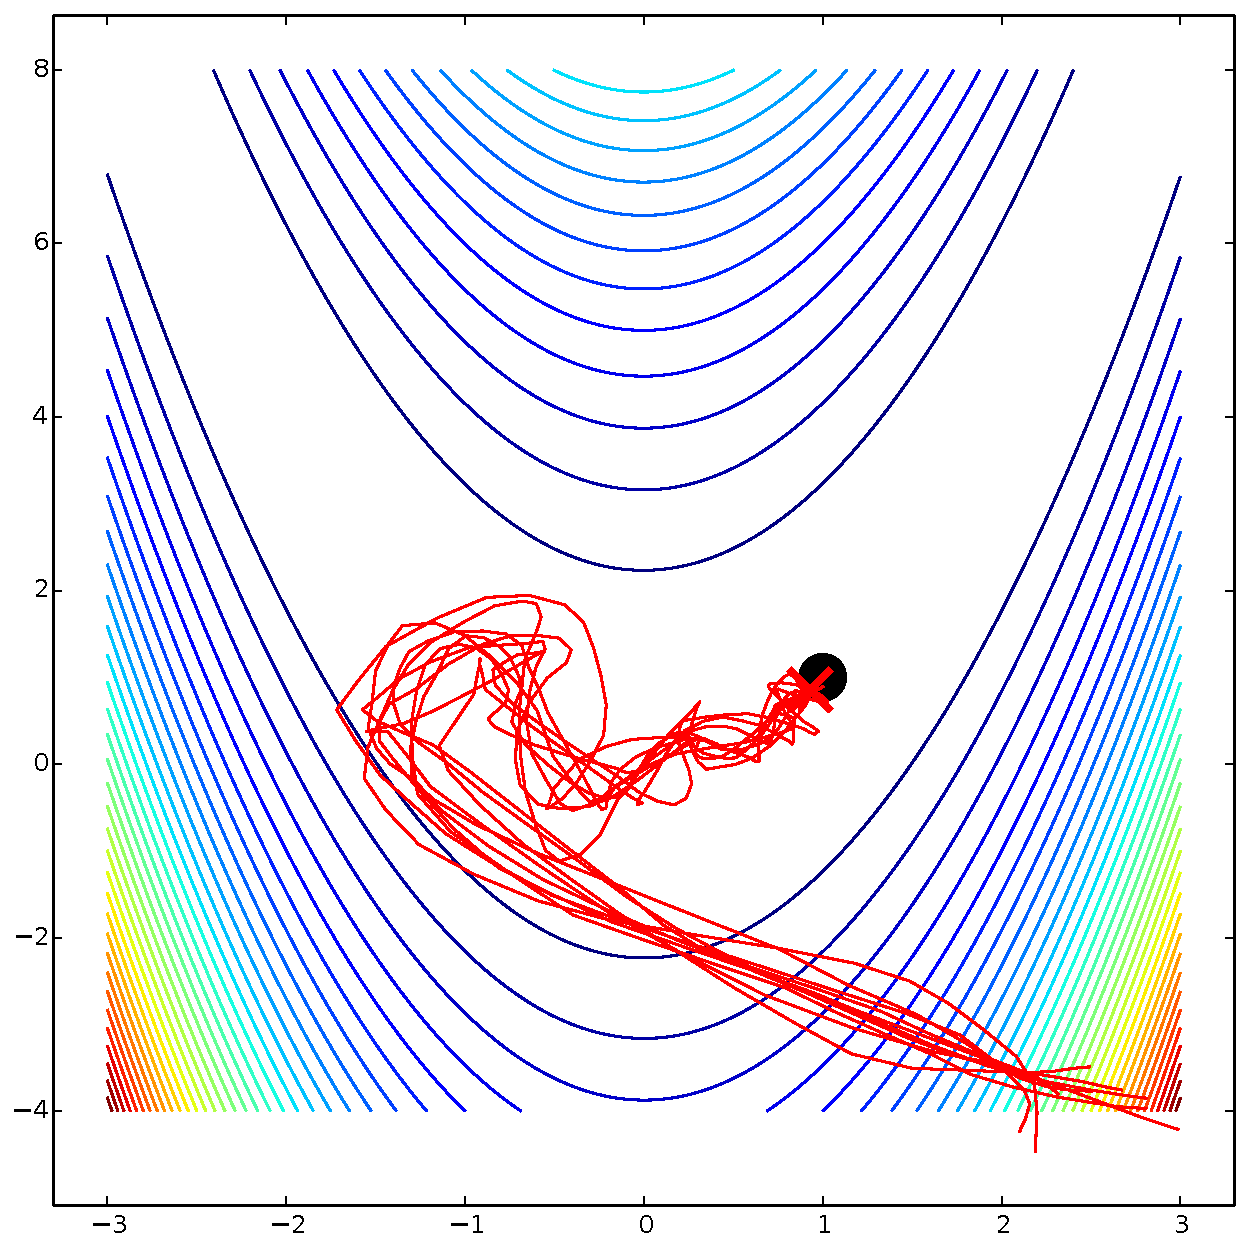
\includegraphics[width=0.45\textwidth]{pso}

    % captions go below figures
    % the optional [] argument is a short version for use in the list-of-figures
    \caption[Particle swarm optimization.]{A particle swarm optimizing the Rosenbrock banana function.}

    % label for referencing figures
    \label{fig:pso}
\end{figure}

\subsection{Subfigures}

In \fref{fig:pso.subfloat}, we again see particle swarm optimization applied to the Rosenbrock banana function.  Now we have two figures, \fref{fig:rosen:banana} and \fref{fig:rosen:pso}.  See the source of this document for sample usage.

% if you have too much margin above your figure, \vspace can move things up
% as a general, however, figures do not have to be exactly flush with the top margin
\vspace{-1em}
\begin{figure}[p!] % p! puts the figure on it's own page
    % use the subfloat to add each figure
    % \\ can be used to start subfigures on the next line
    % or \hfill will fill extra space between side-by-side figures
    \subfloat[The Rosenbrock banana function.]{\label{fig:rosen:banana}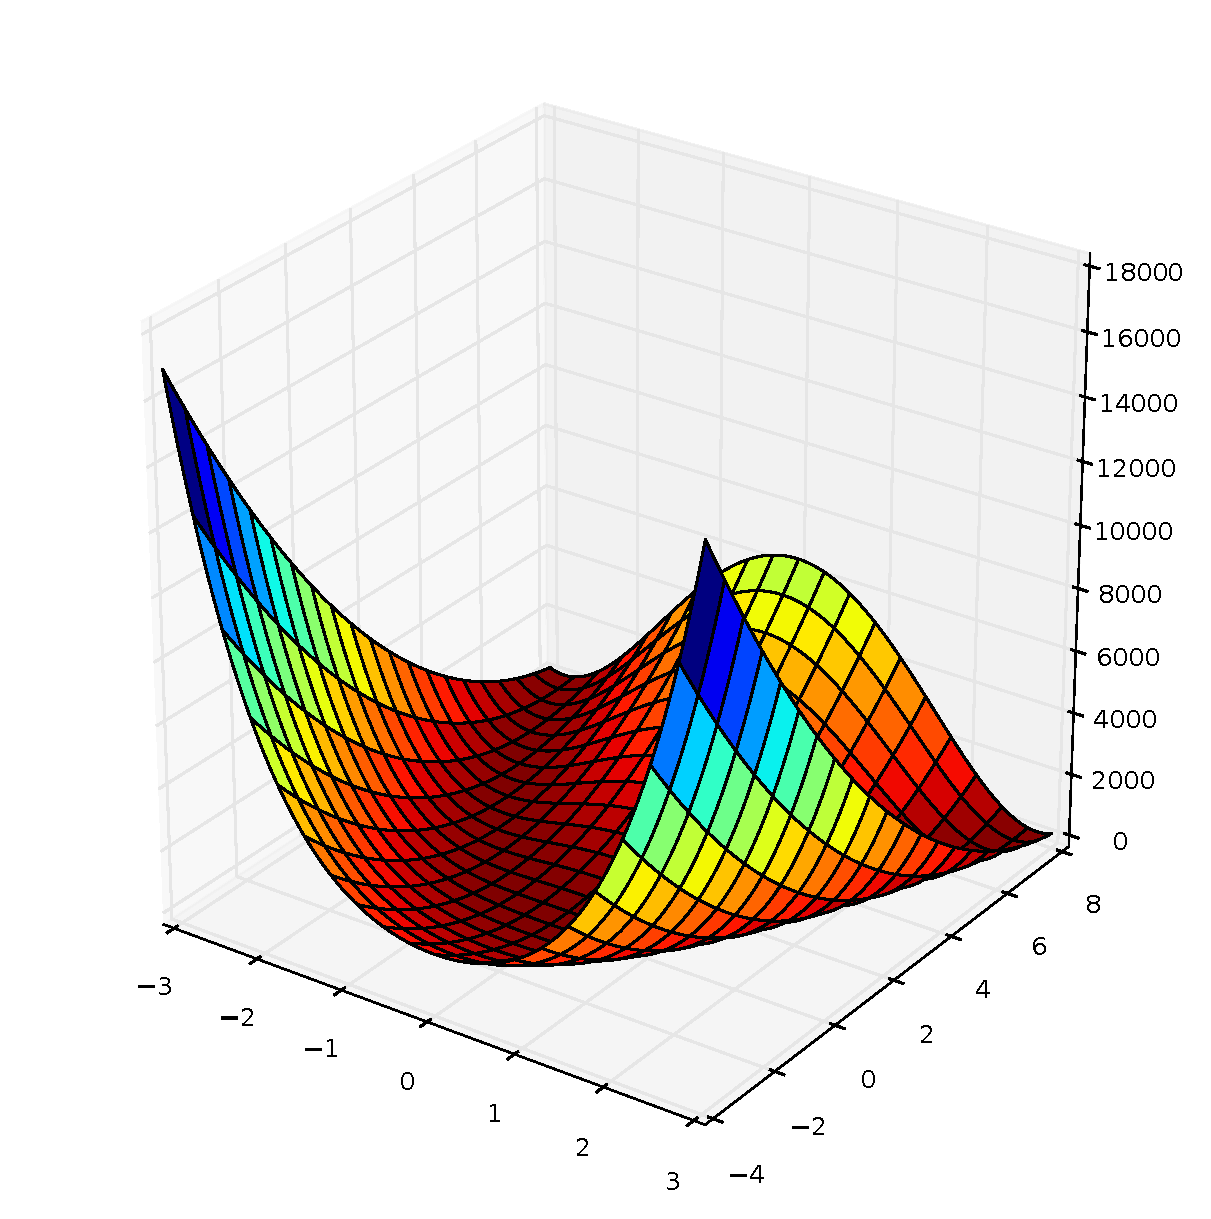
\includegraphics[width=0.45\textwidth]{banana}} \\

    % note that each subfloat can have it's own label
    \subfloat[Path of the particles.]{\label{fig:rosen:pso}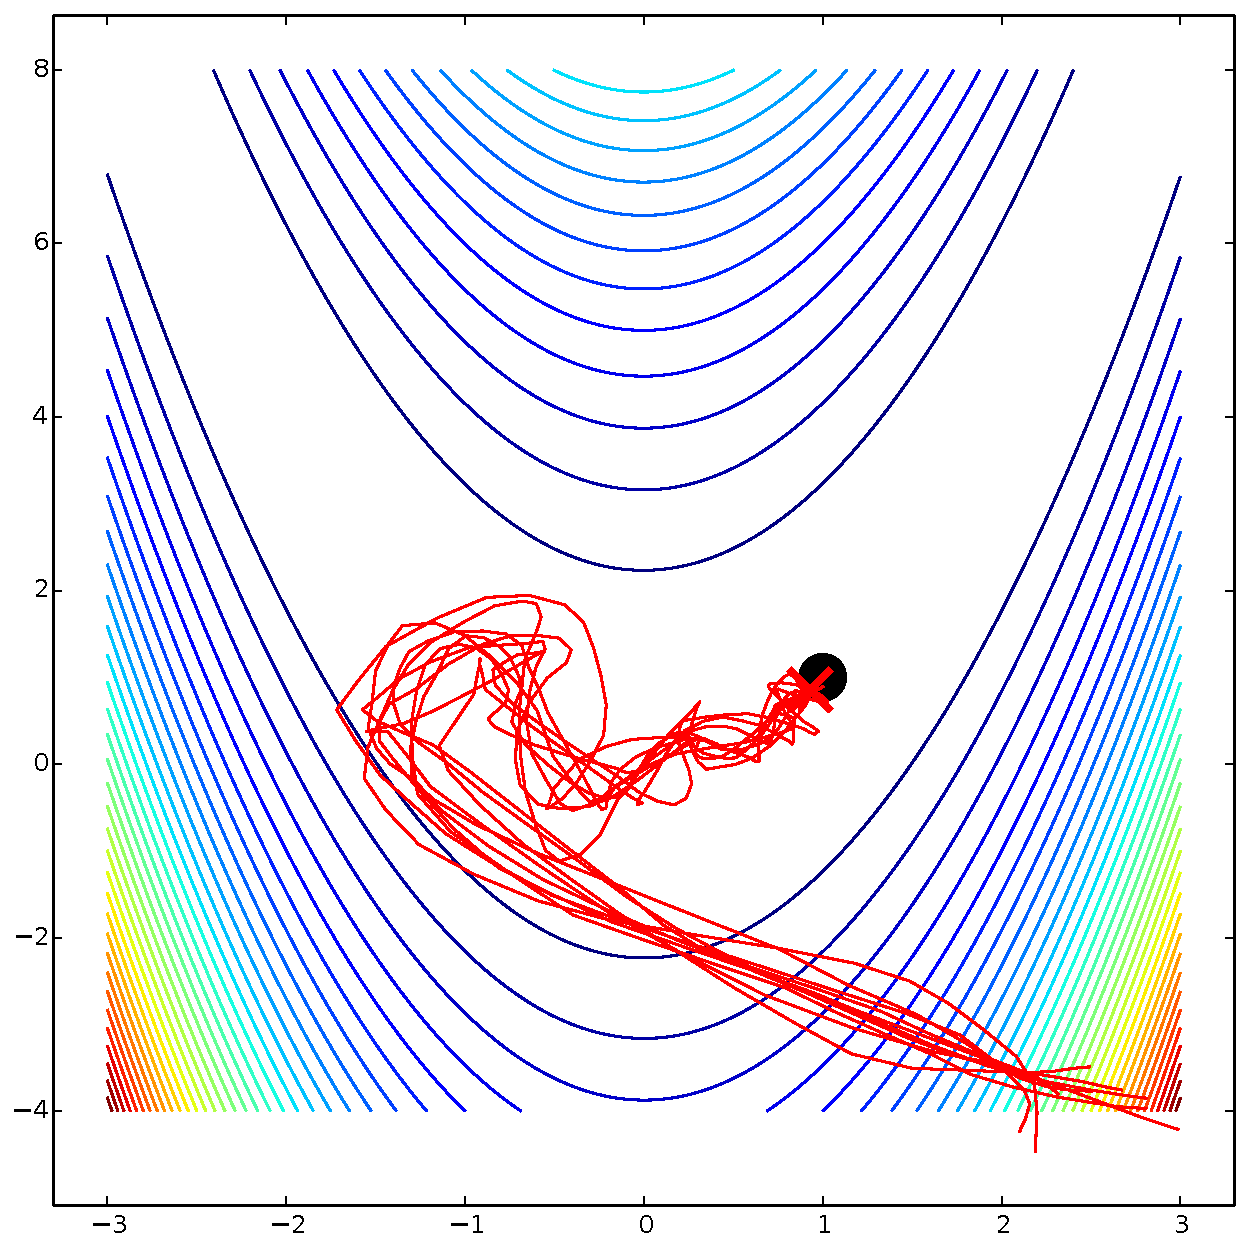
\includegraphics[width=0.45\textwidth]{pso}}

    % the optional [] argument is a short version for the list-of-figures
    \caption[Using PSO to optimize the Rosenbrock banana function.]{Using PSO to optimize the Rosenbrock banana function.  (a)  The function to optimize.  (b)  The path of the particles as they find the global minima.}

    % label for entire figure
    \label{fig:pso.subfloat}
\end{figure}

\section{Sideways Pages}

The thesis guidelines allow horizontal pages for extra wide tables and figures.  \textit{thesis.cls} provides the \textbf{sidewayspage} environment for inserting a single sideways page.  See the source of this document for sample usage.

Note that the sideways page currently needs some work.  If things are too big to fig to fit, it will break and you will need to reduce the size of your figure or table.

\begin{sidewayspage} % if your figures are too big to fig, things will break
    \begin{figure} % don't put [p] here!!
        \subfloat[The Rosenbrock banana function.]{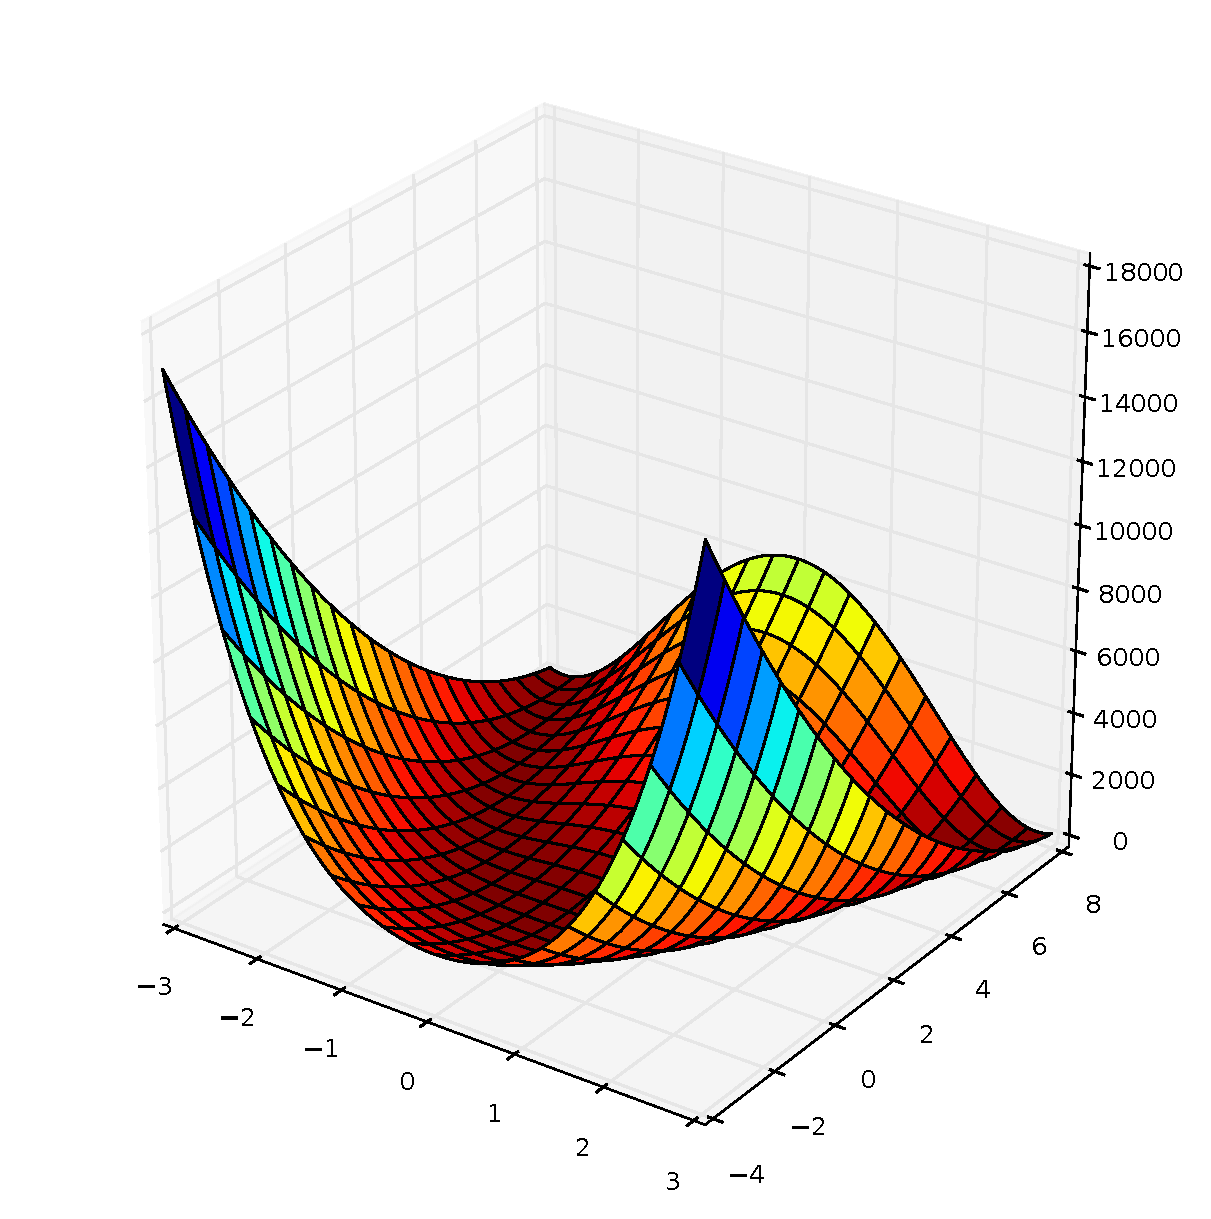
\includegraphics[width=4in]{banana}} \hfill
        \subfloat[Path of the particles.]{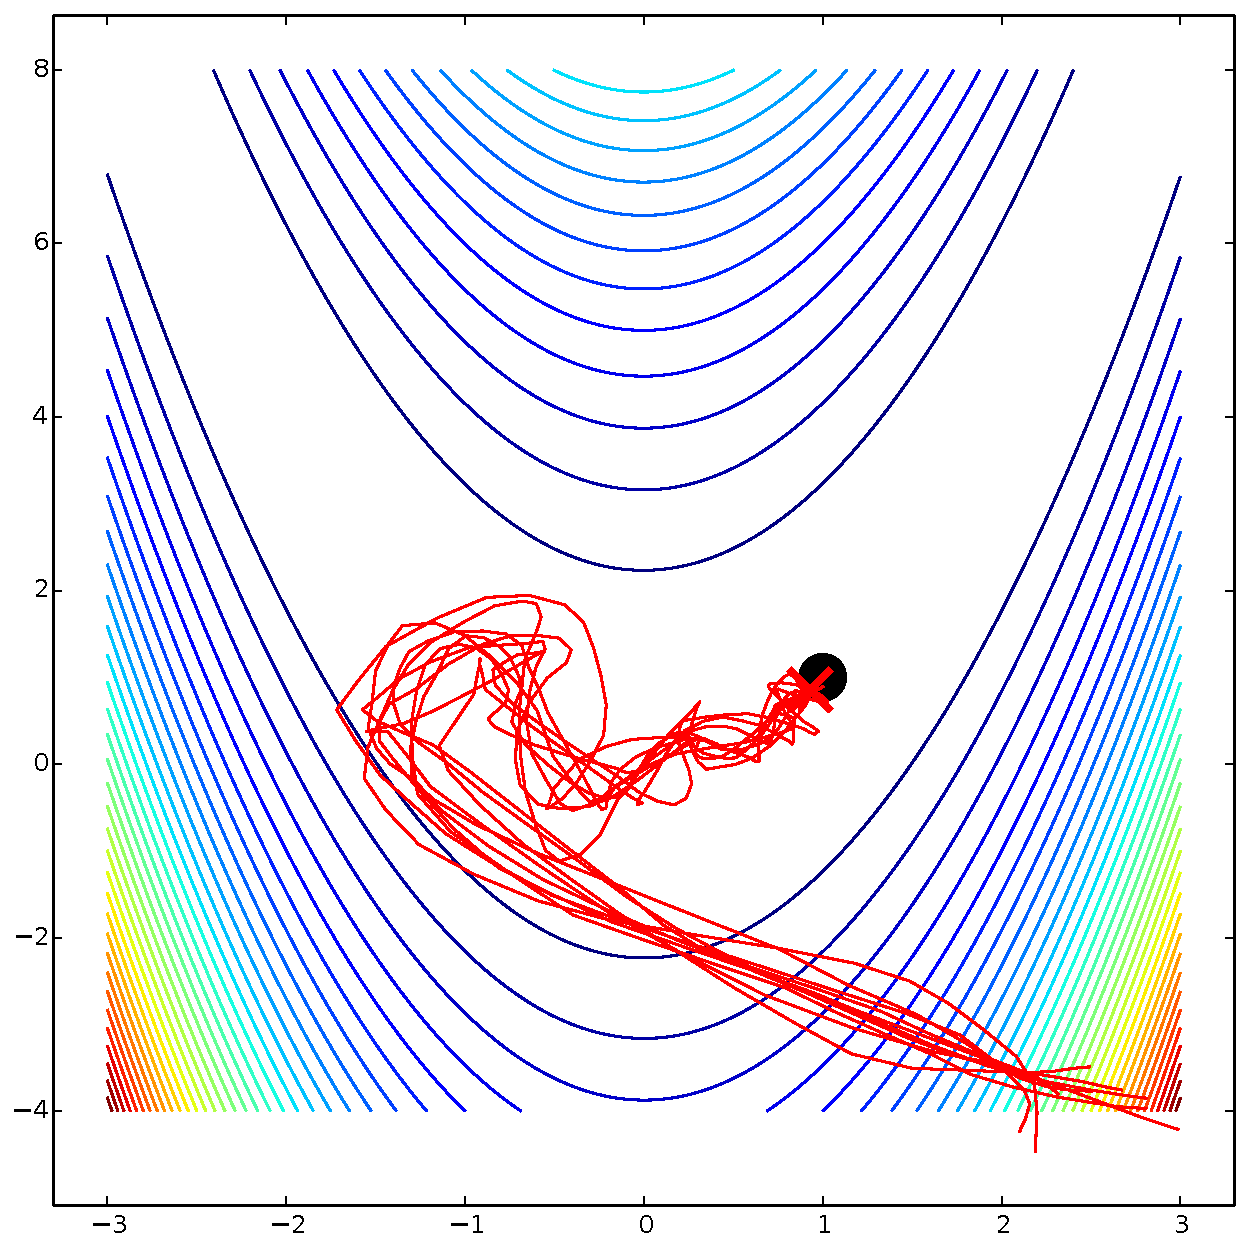
\includegraphics[width=4in]{pso}}
        \caption[PSO on sideways page.]{Using PSO to optimize the Rosenbrock banana function.  (a)  The function to optimize.  (b)  The path of the particles as they find the global minima.}
    \end{figure}
\end{sidewayspage}

\section{Tables}

In \tref{table:sample}, we see an example of a simple table using the \textit{booktabs} package.  Note that other packages are available and allowed for making your tables if you prefer something different.  Table captions go above the table.  See the source of this document for sample usage.

\begin{table}[hp]
    % table captions go above the table!
    % a short version of the caption goes in [] for use in the list-of-tables
    \caption[Sample table.]{A table of groundbreaking results.  The caption goes above the table.}
    \label{table:sample}

    \begin{center}
        \begin{tabular}{@{}*{4}{l}} % four columns, left justified
            \toprule % thick rule at top
            Data-A  & Data-B    & Data-C    & Data-D \\
            \midrule % thin rule in middle
            0.5     & 0.5       & 0.5       & 0.5   \\
            0.5     & 0.5       & 0.5       & 0.5   \\
            0.5     & 0.5       & 0.5       & 0.5   \\
            0.5     & 0.5       & 0.5       & 0.5   \\
            0.5     & 0.5       & 0.5       & 0.5   \\
            0.5     & 0.5       & 0.5       & 0.5   \\
            0.5     & 0.5       & 0.5       & 0.5   \\
            0.5     & 0.5       & 0.5       & 0.5   \\
            \midrule
            Mean    & 0.5       & 0.5       & 0.5   \\
            \bottomrule % thick rule at bottom
        \end{tabular}
    \end{center}
\end{table}

\section{Equations}

Your equations should work as expected.  For example,
\begin{equation}
    \mathbf{z}(t) = \phi(\mathbf{H} \bar{\mathbf{x}}(t) + \mathbf{S} \mathbf{z}(t-1)),
    \label{eq:somefunc}
\end{equation}
where $\mathbf{z}(t)$ is the output of some function at time $t$.  We typically reference equations as \eqref{eq:somefunc}.

\chapter{Creating References and Citations}
\label{chap:references}
%%%%%%%%%%%%%%%%%%%%%%%%%%%%%%%%%%%%%%%%%%%%%%%%%%%%%%%%%%%%%%%%

\section[Citation]{Citation\footnote{This is an example of a citation contained in a footnote \cite{cebl}.}}

The \textbf{\textbackslash cite} command can be used to reference sources from your bibliography.  For example, this sentence cites a number of articles \cite{forney2011classify, cebl, forney2011thesis, forney2015echostate, haykin2009neural}.

The Graduate School requires  ``... any references to journal publications, authors, etc. on your chapter pages or major heading pages [to] be listed as a footnote." This section heading contains an example of such a citation.

\section{Footnotes}

The \textbf{\textbackslash footnote} command can be used to insert footnotes.\footnote{this is a sample footnote.}

\section{Bibliography}

BibTeX is an excellent tool for managing your bibliography and is used in this example.  See the companion \textit{sample.bib} file for examples of how to place entries in your bibliography.  \LaTeX{} will then automatically generate your Bibliography section.

\textit{thesis.cls} is tested with BibTeX and the standard \textit{unsrt} style of references but, in general, other bibliography packages and styles should work.

\chapter{Formatting Tips and Tricks}
\label{chap:tips.and.tricks}
%%%%%%%%%%%%%%%%%%%%%%%%%%%%%%%%%%%%%%%%%%%%%%%%%%%%%%%%%%%%%%%%

\section{Widows and Orphans}

Widows and orphans occur when a single line of text from the beginning or end of a paragraph end up alone at the top or bottom of a page.  Orphans and windows are not allowed in your thesis or dissertation and the graduate school will flag them.  \textit{thesis.cls} sets all possible penalties to attempt to prevent \LaTeX{} from generating orphans and widows.  In some pathological cases, however, they may still occur.  If you find yourself in this position, you have several options:

\begin{enumerate}
    \item Reword your text.  I know, you shouldn't have to change your text for formatting purposes, but often this is the easiest way.

    \item Change the size of a figure or table or shift things around a bit.

    \item Insert a \textbf{\textbackslash clearpage} command to start the next page directly before the culprit paragraph.

    \item Try tweaking the values of \textbf{\textbackslash clubpenalty} and \textbf{\textbackslash widowpenalty}.  Note, however, that this might cause widows and orphans to spring up elsewhere in your document.
\end{enumerate}

\section{Margins}

The graduate school is very strict about enforcing 1'' margins.  Before submitting your thesis, try passing the \textbf{showframe} argument to \textit{thesis.cls}.  This will show a frame around each page that will help you troubleshoot your margins.  If you see anything outside this box, be sure to fix it.

Note that figures and tables do not have to be perfectly flush with the margins but cannot violate them.  Note, however, that figures often have an extra margin built in from the program that generated the plot.  These margins can lead to large extra spaces that are occasionally flagged by the graduate school.  Try and remove the margins when you generate your figures.  Alternately, look at tools like inkscape, gimp or photoshop for trimming the margins in your figure files.

\sloppy
If you have a very long word that flows into the side margin,\footnote{this should generate an ``overfull hbox badness'' warning} you can typically correct the problem by applying the \textbf{\textbackslash sloppy} command to a single paragraph.  This will loosen the \LaTeX{} typesetting rules and allow the margin requirements to be met.  See this paragraph in the source of this document for an example.  Note that you should reverse the effects of sloppy using the \textbf{\textbackslash fussy} command at the end of the paragraph.  Using sloppy rules everywhere will lead to odd-looking spacing.
\fussy

\backmatter % starts unnumbered supplementary material
%%%%%%%%%%%%%%%%%%%%%%%%%%%%%%%%%%%%%%%%%%%%%%%%%%%%%%%%%%%%%%%%

% Bibliography
%%%%%%%%%%%%%%%%%%%%%%%%%%%%%%%%%%%%%%%%%%%%%%%%%%%%%%%%%%%%%%%%

% unsorted BibTeX style
% check here for more:  https://www.sharelatex.com/learn/Bibtex_bibliography_styles
%\bibliographystyle{apacite} % apa style bibliography
\bibliographystyle{unsrt} % math and engineering style bibliography

\bibliography{sample} % change sample to the name of your .tex file, e.g., thesis

\appendix % starts the appendices
%%%%%%%%%%%%%%%%%%%%%%%%%%%%%%%%%%%%%%%%%%%%%%%%%%%%%%%%%%%%%%%%

\chapter{License}
\label{appendix:license}
%%%%%%%%%%%%%%%%%%%%%%%%%%%%%%%%%%%%%%%%%%%%%%%%%%%%%%%%%%%%%%%%
{
    % this formatting is just for the license,
    % no need for this in your appendix
    \setlength{\parindent}{0em}
    \setlength{\parskip}{1em}

    \textbf{Colorado State University LaTeX Thesis Template}

    by Elliott Forney -- 2017

    This is free and unencumbered software released into the public domain.

    Anyone is free to copy, modify, publish, use, compile, sell, or distribute this software, either in source code form or as a compiled binary, for any purpose, commercial or non-commercial, and by any means.

    In jurisdictions that recognize copyright laws, the author or authors of this software dedicate any and all copyright interest in the software to the public domain. We make this dedication for the benefit of the public at large and to the detriment of our heirs and successors. We intend this dedication to be an overt act of relinquishment in perpetuity of all present and future rights to this software under copyright law.

    THE SOFTWARE IS PROVIDED "AS IS", WITHOUT WARRANTY OF ANY KIND, EXPRESS OR IMPLIED, INCLUDING BUT NOT LIMITED TO THE WARRANTIES OF MERCHANTABILITY, FITNESS FOR A PARTICULAR PURPOSE AND NONINFRINGEMENT.  IN NO EVENT SHALL THE AUTHORS BE LIABLE FOR ANY CLAIM, DAMAGES OR OTHER LIABILITY, WHETHER IN AN ACTION OF CONTRACT, TORT OR OTHERWISE, ARISING FROM, OUT OF OR IN CONNECTION WITH THE SOFTWARE OR THE USE OR OTHER DEALINGS IN THE SOFTWARE.
}

% Have a nice day!
%%%%%%%%%%%%%%%%%%%%%%%%%%%%%%%%%%%%%%%%%%%%%%%%%%%%%%%%%%%%%%%%
\end{document}
